    
\section{Introduction}

This chapter sheds light on the overarching theme of this project - The Third Space - by looking at the current work done in this particular domain by reviewing academic articles and papers.

As introduced in above sections, this project aims to target two sub domains, i.e. Rights and Employment Opportunities of marginalized communities and market condition(s) of small-scale Arts and Crafts businesses. Therefore, this Literature Review, while taking into account the current state(s) and other similar work that has been done in the area of art and crafts and employment opportunities for marginalized communities, also establishes the novelty of our work by highlighting the differences between the existing work and our work.

This Review will comprise of statistics taken from the cited literature as well as an analysis of primary text. We'll first review the literary sources catering to the domain of the plight of marginalized communities. Followed by this will be the review of the literary sources related to the Pakistani handicraft industry which will then lead to our discussion of rising e-commerce industry in Pakistan.

There are a large number of studies about the transgender communities and much is known and written about 'hijras' (transgender persons) in India, however, very little is documented about them in Pakistan (Jami, 2005). It is also to note that the focus of this research is the sad state of these communities with regards to their rights and employment opportunities, therefore this research will use the umbrella term `transgender' instead of going into the depth of multiple terms ('Zanana', 'Khuwaja Sira', 'Mukhannas', 'Hijra') used within South Asian culture (Winter, 2002). 

\section{Conceptual Frame Work}

This is the high level Conceptual Framework for this project. We have two types of variables here, i.e. independent and dependent variables. The rectangle shaped variables in the given figure is the independent variable while the Eclipse shaped variable is the dependent one.

\begin{figure}
  \caption{Conceptual Framework of the research project}
  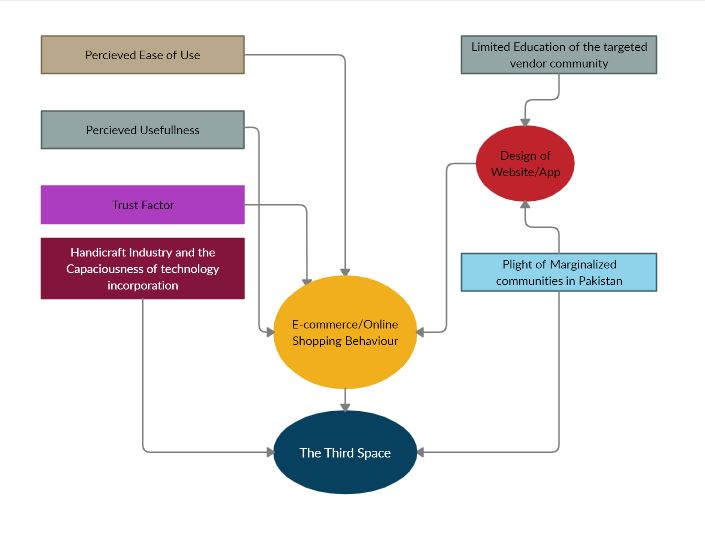
\includegraphics[width=0.75\textwidth]{Conceptual Framework.JPG}
  \centering
\end{figure}

\section{Theoretical Frame Work}

\section{Emperical Review of Previous Work(s)}

In this section, we'll look at the research work done already by local and international researchers in the three domains our project is related with. This section will take on these three domains in chronological order and discuss the various researchers' works  and the results they arrived while also putting them in context.

\subsection{The state of Pakistan's marginalized communities}

There is limited literature based on primary data of transgender persons in Pakistan (Nazir \& Yasir, 2016). Just the factor that we have little to no documentation for an entire community in relation to their population, literacy rate, employment rate, etc. is telling enough as to how our society has devoid them of any rights. This is the particular reason why the author(s) of this report chose to work in this domain. The need for this cause to be taken up by scientists and engineers today is far more important so that we can find solutions with the aid of technology and create a better world for all of us. 

In a research done by Jami, H. in 2005 with the name \textit {Condition and status of hijras (transgender, transvestites etc) in Pakistan}, she concludes that,“ `We hate some people but we do not know them and we do not want to know them because we hate them', this dictum stands valid in our attitude towards hijras." This research concludes that the discriminating attitude is in effect by and large in our society against the personalities of transgender communities. It can also be drawn from the study that not only Pakistanis have the instilled bias against the transgender persons and people detest the idea of having a transgender in a family, but they are also considered responsible for sex business and homosexuality (Jami, 2005) both of which in a society as religiously conservative as Pakistan's, are considered blatant sins and is also one of the root causes of violence against the member of these communities. This study also confirms that women tend to have positive attitude towards transgender persons compared to men (who are also the performers and executers of violence on the members of this already marginalized community). 

Another research done by Tabassum, S. \& Jamil, S. in (2014) by the title of \textit {Plight of marginalized: Educational issues of transgender community in Pakistan} also affirms the same as Zubaida (a trans woman) states “Brothers and fathers never bother to think about our (transgender person) situation perhaps they thanked to God if we left the home”. Tabassum \& Jamil also concludes in their study that there is a greater desire (of almost 94\% of the sample population from the community) to acquire education and it's their belief that education is a necessary tool for their upwards mobility. However, it was also gathered that some of them who tried to get education faced lot of problems in terms of their enrollment in schools, group selection in the class rooms and in answering the unknown questions of the fellows (Tabassum, S., \& Jamil, S., 2014). 

The findings from the research conducted by Nazir, N., \& Yasir, A. in 2016 in the northern province of Pakistan by the title \textit {Education, Employability and Shift of Occupation of Transgender in Pakistan: A Case Study of Khyber Pakhtunkhwa.} showed that transgender people have experienced unemployment twice the rate of the population as a whole. 97\% of the surveyed population was facing mistreatment on the job. Out of total 47\% faced an adverse job outcome, including job refusal, or being fired or denied promotion. 26\% lost their job because of being transgender. 15\% of the sampled respondents lived in poverty which was double the rate of the general population (Nazir \& Yasir, 2016). This study also talks about the stigma attached to the families of transgender persons and how society continuously taunts them till they disown their child which leads them to being deprived of normal life, education and later on earning means that are considered honorable in the society (Nazir \& Yasir, 2016). It is also to note that this report also talks about the landmark judgment by the Supreme Court of Pakistan which directed both federal and provincial governments to ensure the rights of education, employment and inheritance (Nazir \& Yasir, 2016). Yet, the measures taken by the state in accordance with the court's ruling are not concrete enough to provide the support they need.

Contextualizing the above findings of all of these reports, we can easily draw the conclusion that the community under consideration is one of the many marginalized communities in our society and there are various factors acting behind this sad state of affairs. Therefore, the need for such a project which could create employment opportunities for them is due well in time.

\subsection{The state of Pakistan's handicraft industry}

We begin by deconstructing the term 'handicraft'. Different researchers have described it didfferently. For example, Fabeil (2014) describes that Handicraft refers to handmade products that have artistic and cultural attraction based on their material, design and workmanship. Whereas, Rogerson (2010) attests that craft products should be eighty percent (80\%) made by hands that may include various raw materials such as natural fibers, textiles, beads clay and recyclable materials. However, Thompson (1995) and Abryareh (2006) defines handicraft as a skill, specifically involving practical arts. Most of the debate about definition is on how product is made (handmade versus machine-made, simple versus artistic qualities etc. but the understanding of it as a means of cultural preservation and money-generating economic option is established.

The handicraft sector plays a vital role in income and employment generation and has also been recognized worldwide as a tool for poverty reduction (Allal \& Chuta, 1982). It is a means of preserving and promoting cultural and artistic traditions, such as various techniques and skills of traditional crafts are transmitted from generation to generation. For many countries, the significant unique cultural heritage is retained in their handicrafts, concluded Allal, M., \& Chuta, E. in 1982 in their research by the title \textit {Cottage industries and handicrafts; some guidelines for employment promotion.}

In an extensive study undertaken by a team of British Council (a worldwide cultural organisation of United Kingdom) with the title of \textit {Mapping cultural and creative industries in Pakistan}, the handicraft industries in context with Pakistani society is looked upon in depth. It is concluded in the study that although handicrafts lie in the hemisphere of culture and creativity, the idea of culture and creativity being an evolving industrial activity with wider social, economic and cultural impacts is one which has developed over a long period of time.

In another research by Yang, Y., Shafi, M., Song, X., \& Yang, R. in 2018 by the title of \textit {Preservation of cultural heritage embodied in traditional crafts in the developing countries. A case study of pakistani handicraft industry}, the rise and fall of Pakistani handicraft making as an industry and the impact(s) of technological advancement on this sector. The handicraft trade at global level is focused on customer’s needs and tastes instead of trade in culture. The production of handmade products in bulk quantities, requires mechanical support for finishing and processing. Moreover, the artisan needs to produce innovative designs, shapes, color etc. to match the needs of customers and such innovation may not contain traditional flavor. In Pakistan, several studies indicate that handicraft producers have a low level of education. One of the major reason of low education is that various products require complex and lengthy process and often involves whole family including children which means children quit or miss the school. This is one of a challenging constraint in preserving craft tradition as low level of education makes it difficult for artisan to access various government schemes, obtain market information, bargain with middlemen/traders and manage business properly, thus making them uncompetitive. Moreover, the number of vocational institutes providing training in handicraft skills is very small in various countries such as the case of Laos, there is only one vocational training school (Yang, Shafi, Song, \& Yang, 2018). It is also to note  that the handicraft industry is considered as a low technology sector which involves traditional methods of production and designs. According to prior studies, the handicraft producers lacked the capability to design and develop new products, therefore they are unable to create the marketable product.

Nowadays, customers have rapidly changing demand for new designs; in order to compete in market, the crafts worker should understand the changing needs of customers and should introduce modern designs, however, the traditional design motif should be preserved. Due to lack of innovation and technology the artisans are unable to meet the demands of the customers (Yang, Shafi, Song, \& Yang, 2018). The innovation is a transformation of ideas and knowledge into new products or services which involve technology and the organization, and can be in terms of production, services, processes or management (Ramadani, \& Gerguri, 2011). Culture can also be preserved through innovation in small businesses (Dana, 1999). As a result, entrepreneurs play a crucial role to ensure that the handicraft industry and its cultural identity are preserved for future generations. Even though the human interaction cannot be simply replaced by the technology, there is significant scope to develop activities that not only document and preserve the knowledge of craftsmanship but also ensure the transmission of this knowledge to younger generations. Moreover, in order to enhance the productivity and efficiency of craft production, technology can be used. Using technology, another way to distinguish handicraft products is to put story behind the unique features, the way it is made, origin of product’s design or the artisans and their culture. Such stories can be attached through digital marketing techniques. This will not only help to distinguish, improve sales but will also help to increase the value of product due to its uniqueness from other substitute products. In addition, it is also one of best way to educate customers about the crafts.

In her thesis report, \textit {The Contemporary Value Chain}, Zahra, S. Virsa also concluded that one of reason behind decline in Pakistani handicraft industry is the lack of innovation in design and emphasized that artisans should adopt modern tastes of customers to compete in the market. Also, there is a wide gap of cooperation between designers and artisans, the designers have the professional knowledge and knowhow about the modern taste and artisans have cultural heritage skills and knowledge, thus their cooperation can lead to expansion of business and competitiveness.

In light of the above-mentioned works, it can be seen that the need of amalgamation of craft industrywith technology can actually pull off a competitive and profitable entrepreneurial venture, which our project aims to be.




\subsection{The state of Pakistan's rising E-commerce in Pakistan}

'Since fake e-stores, cybercrimes and scam websites are very common in Pakistan, people hesitate to shop online.' (Adnan,  2014, p.1). The paradoxical state of Pakistani E-commerce industry is itself a 

\section{Overview of Literature}

\section{References}

\begin{itemize}
     

\item Jami, H. (2005, July). Condition and status of hijras (transgender, transvestites etc) in Pakistan. In Sexualities, Genders and Rights in Asia’, 1st International Conference of Asian Queer Studies Retrieved September (Vol. 5, p. 2006).

\item Sharma, S. K. (2000). Hijras: The labelled deviance. New Delhi: Gyan Publishing House.

\item Talwar, R. (1999). The third sex and human rights. New Delhi: Gyan Publishing House

\item Winter, S. (2002). Transgender Asia. Retrieved June 21, 2004 from http://web.hku.hk/~sjwinter/TransgenderAsia/index.html

\item Nazir, N., \& Yasir, A. (2016). Education, Employability and Shift of Occupation of Transgender in Pakistan: A Case Study of Khyber Pakhtunkhwa. Dialogue (Pakistan), 11(2).

\item Tabassum, S., \& Jamil, S. (2014). Plight of marginalized: Educational issues of transgender community in Pakistan. Review of Arts and Humanities, 3(1), 107-122. 

\item CSS Forum. (2010). Why is there no Status of the Third Gender in Pakistan. Retrieved from http://www.cssforum.com

\item Allal, M., \& Chuta, E. (1982). Cottage industries and handicrafts; some guidelines for employment promotion. International Labour Office.

\item Abryareh, R. (2009). Tourism Attractions and their Influences on Handicraft Employment in Isfahan. Master’s Thesis, Lulea University of Technology.

\item Simon, T. Miranda. (1995). The Craft of Functional Programming; Addison-Wesley Longman Publishing Co.

\item Rogerson, C.M. (2010). The Enterprise of Craft: Constraints and Policy Challenges in South Africa. Acta Acad. 42, 115–144.

\item Fabeil, N.F., Pazim, K.H.; Marzuki, K.M.; Langgat, J. (2014). The orientation of handicraft entrepreneurs in Sabah: Their personality characteristics and motivations (Orientasi Usahawan Kraftangan di Sabah: Ciri Personaliti dan Motivasi). In Proceedings of the 2nd ASEAN Entrepreneurship Conference, Penang, Malaysia.

\item Fatori´c, S., Seekamp, E. (2017). Securing the Future of Cultural Heritage by Identifying Barriers to and Strategizing Solutions for Preservation under Changing Climate Conditions. 

\item Simon, T. Miranda. (1995).The Craft of Functional Programming; Addison-Wesley Longman Publishing Co.

\item Ramadani, V. \& Gerguri, S., (2011).  Theoretical framework of innovation: Competitiveness and innovation program in Macedonia.

\item Zahra, S. Virsa, (2015). The Contemporary Value Chain. Master’s Thesis, Virginia Commonwealth University.

\item Dana, L.P. (1999). Preserving culture through small business: Government support for artisans and craftsmen in Greece. 

\item Yang, Y., Shafi, M., Song, X., \& Yang, R. (2018). Preservation of cultural heritage embodied in traditional crafts in the developing countries. A case study of pakistani handicraft industry. Sustainability, 10(5), 1336. https://www.mdpi.com/2071-1050/10/5/1336

\item Evans, K., Stockley, S., Taylor, C., Brown, J., Rab, M., \& Khan, S. (2014). Mapping cultural and creative industries in Pakistan. 


\end{itemize}
Of course, we take inspiration from \cite{einstein} but wish the work was typeset in \LaTeX \cite{knuthwebsite}, e.g. by taking help from \cite{latexcompanion}.